\documentclass[journal=jprobs,manuscript=article,layout=traditional]{achemso}

\usepackage[T1]{fontenc}

\usepackage[utf8]{inputenc}

\usepackage{graphicx}

\usepackage{amsmath}

\usepackage{booktabs}
\usepackage{url}

\usepackage{lmodern}

\SectionNumbersOn

\author{Murat G\"ok}

\affiliation{Department of Computer Engineering, Faculty of Engineering, Yalova University, 77200 Yalova, T\"urkiye}

\email{murat.gok@yalova.edu.tr}

\title{Condition identity and label weighting govern structure-response inference from reused site-resolved PTM data: a reanalysis of enzymatic carboxymethyllysine repair}

\keywords{proteomics data reuse, post-translational modification, carboxymethyllysine, label construction, inverse-variance weighting, structural bioinformatics}

\sloppy
\begin{document}

\begin{tocentry}

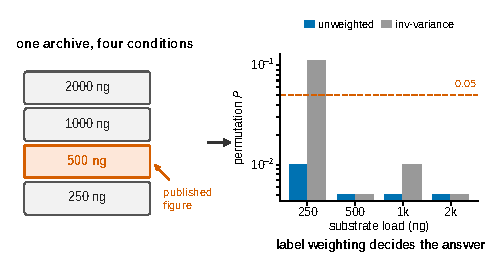
\includegraphics[width=\linewidth]{figures/toc_graphic.pdf}

\end{tocentry}

\maketitle

\begin{abstract}

Site-resolved measurements of how a post-translational modification responds to an enzyme are increasingly reused as labels for computational models, but little is known about how robust such labels are to the analytical choices made when deriving them. We examined this using ProteomeXchange PXD070124~\cite{trabosh2026a,trabosh2026b}, which accompanies the first report of an enzyme that reverses~\cite{trabosh2026a} $N^{\varepsilon}$-carboxymethyllysine and deposits site-level quantification for four substrate loads. The published site-level figure reports one load without stating which; we identify it as the 500 ng condition from replicate-level agreement, the number of sites passing the confidence threshold, and the number of highly responsive sites. Converting active-versus-control abundance ratios into inverse-variance sample weights, a natural choice given the available delta-method variance, proved harmful: the weights spanned up to five orders of magnitude, the Kish effective sample size~\cite{kish1965} fell to 0.23-0.32 of the nominal site count, and a structure-response relationship was recovered in three of four conditions under weighting against four of four without it. Clipping the weights did not repair this. The mechanism is that the delta-method variance carries the control mean in its denominator, so low-occupancy sites are systematically downweighted. Unweighted, local structural descriptors carried permutation-controlled predictive information in all four loads (P = 0.010, 0.005, 0.005, 0.005). The relationship was not uniform across sites: the twenty lysines quantified confidently at every load showed no signal in any condition, at the third percentile of random-subset resampling, which excludes loss of power. Reuse of ratio-based site-level response data therefore requires that the reporting condition be stated and that inverse-variance weighting be justified rather than assumed.

\end{abstract}

\section{Introduction}

Site-resolved proteomics increasingly supplies~\cite{disanzo2021a} not only maps of where a post-translational modification occurs, but quantitative measurements of how individual modified residues respond to a perturbation. Such measurements are attractive as labels for computational models, because they promise to turn a chemical modification into a per-residue phenotype. They are also scarce, small, and produced under conditions chosen for the original experiment rather than for reuse. How robust they are to the analytical choices a secondary user must make has not, to our knowledge, been examined on a real dataset.

Prediction of lysine glycation from sequence and structure is itself an established line of work, running from early neural-network classifiers through structure-aware support vector machines to recent transformer-based models~\cite{johansen2006,reddy2018,yu2019,liu2022,jia2024}. Every one of these predicts occurrence: which lysines carry the modification. None predicts how a modified lysine responds to an enzyme, because until recently no such measurements existed. Response labels are therefore a new and largely unexamined class, and the question of how robustly they can be derived from a deposition has not been asked.

$N^{\varepsilon}$-carboxymethyllysine (CML) provides an unusually clean test case. Chemically stable and abundant in long-lived proteins~\cite{chaudhuri2018}, CML was treated as a terminal modification: endogenous defences such as the glyoxalase system and fructosamine-3-kinase~\cite{schalkwijk2020} act on precursors or early glycation adducts, and the reported deglycase activity of DJ-1/PARK7 remains contested~\cite{richarme2015}. The recent description of an engineered FAD-dependent oxidase that oxidises the $N^{\varepsilon}$-carboxymethyl group and restores native lysine therefore created the first site-level response measurements for this modification class, together with a public deposition.

The source study reported that of thirty-three CML-modified lysines detected on bovine serum albumin, thirty showed reduced CML, and it noted qualitative structural trends: activity was "not strictly a function of surface accessibility", three lysines in surface-exposed helices "showed varied CML reductions of 90\%, 38\%, and 0\%", activity "weakly correlated with local protein flexibility (B-factor)" such that "flexibility may be necessary but is not sufficient for catalysis", and "some local sequence preference was observed, with CMLase showing higher activity on sites with neighboring cysteines" while "reduced enzymatic activity was associated with bulky hydrophobic or aromatic residues". The legend of the corresponding figure nonetheless states that the enzyme "has varying activity across all sites with no clear preference based on primary or secondary structure". These observations are the starting point for the present work rather than a gap in it: the structural hypotheses have been stated, and what is missing is a quantitative test of whether they survive the choices a reuser must make.

Those choices turn out to be consequential, and they are the subject of this paper. The deposited dataset contains processed site-level quantification for four substrate loads, whereas the published site-level figure reports one of them without identifying it. A response defined as one minus the ratio of active-enzyme to inactive-control abundance has a readily computed delta-method variance, which invites inverse-variance weighting. And the set of lysines that pass an identification-confidence threshold differs between loads, so the site composition of a label set is itself a function of the condition from which it was taken.

We therefore treat the reuse operation as the object of study. We identify which condition the published figure reports, reproduce it with an independent implementation, and then ask how the apparent structure-response relationship depends on the weighting scheme, on the substrate load, and on which sites are included. The structural model is a vehicle for these questions rather than a contribution in itself; the descriptors and the regressor are standard, and we make no claim about proteome-wide repairability or transfer to other scaffolds.

\section{Experimental Section}

\subsection{Scope and reuse design}

The study is a secondary computational analysis of publicly deposited proteomics data. No new mass-spectrometry, biochemical, cell, animal or human experiments were performed, and no raw spectra were reprocessed: the deposited dataset provides processed site-level quantification, and we used it as deposited. The claim boundary was fixed before analysis. We asked whether local structural descriptors carry reproducible information about site-specific CML reduction within bovine serum albumin, and we treated condition-level replication as the primary test. We make no claim about proteome-wide repairability, about enzyme delivery, or about transfer to other protein scaffolds.

\subsection{Data source and condition identification}

Site-level quantification was taken from ProteomeXchange dataset PXD070124, files ~\cite{perezriverol2025}\texttt{BSA\_\allowbreak \{0p25,0p5,1p0,2p0\}\_\allowbreak 865\_\allowbreak 794\_\allowbreak processed\_\allowbreak filt\_\allowbreak quant.csv}. SHA-256 prefixes of the four files are reported in the data availability statement. Each file reports, per lysine, the protein, residue number, modification, peptide sequence, an identification confidence score, and percent abundance for three active-enzyme and three inactive-control replicates. The four files correspond to the four substrate loads described in the source report, in which 250, 500, 1000 or 2000 ng of CML-modified BSA in a 25 uL reaction was incubated with enzyme at fixed concentration; the enzyme-to-substrate ratio therefore falls as load rises. Residue numbering in the deposited files is UniProt numbering~\cite{uniprot2025} for P02769, which we confirmed against the mature-chain offset of 24 used in the source analysis.

The source report does not state which substrate load its site-level figure represents. We identified it as the 500 ng condition on three independent grounds, reported in Results: exact agreement of replicate-level percent abundance values with the figure source data, agreement of the number of sites passing the confidence threshold, and agreement of the number of sites showing more than ninety percent reduction. Sites were retained when the identification confidence score exceeded 90, the threshold used in the source analysis.

\subsection{Site-level response labels and the weighting decision}

For each site in each condition the response was defined as one minus the ratio of the active-enzyme mean percent abundance to the inactive-control mean percent abundance, computed from the three replicates on each arm and truncated to the unit interval. Sites with a control mean of zero were excluded because the ratio is undefined. Truncation affected a small number of sites per condition (two, one, five and three at 250, 500, 1000 and 2000 ng), and the number of sites at the lower and upper boundary after truncation is reported in Results. The endpoint is a relative reduction in CML signal under one assay and is not interpreted as an intrinsic probability that a site is repairable.

An approximate variance was obtained for each response by the delta method, combining the replicate-mean variances of the two arms as $\mathrm{var}(A)/C^{2} + A^{2}\,\mathrm{var}(C)/C^{4}$, where A and C are the active and control means. The source pipeline converted these variances into inverse-variance sample weights. We evaluated that choice rather than inheriting it, and we did not retain it.

Three observations motivate the decision. First, the weights are extremely skewed: within a condition they span roughly three to five orders of magnitude, and the Kish effective sample size falls to between 0.23 and 0.32 of the nominal site count, so the thirty-three nominal sites of the published condition correspond to an effective sample of 9.7. Second, the weighting suppresses the structure-response relationship: under inverse-variance weighting the permutation-controlled signal was recovered in three of four conditions, whereas without weighting it was recovered in all four, with higher rank correlations in three of the four. Third, clipping the weights to a moderate range reproduced the weighted outcome rather than the unweighted one, which indicates that the problem is the direction of the weighting rather than a few extreme values.

The mechanism is specific to ratio-based response labels. The delta-method variance carries the control mean in the denominator, so sites with low control abundance receive large variances and correspondingly small weights. Low occupancy, however, is a property of the site rather than noise about the structure-response relationship, so inverse-variance weighting systematically downweights low-occupancy sites and introduces an occupancy-dependent bias. We therefore report unweighted analyses as primary and inverse-variance and clipped weighting as sensitivity analyses, and we recommend that reuse of ratio-based PTM response labels treat inverse-variance weighting as a modelling choice requiring justification rather than a default.

\subsection{Structural descriptors}

Structural features were extracted from the crystallographic model of bovine serum albumin, PDB 4F5S~\cite{bujacz2012}, chain A. Solvent-accessible surface area was computed with the Shrake-Rupley algorithm~\cite{shrake1973} and normalised to the residue-specific maximum accessibility scale for lysine~\cite{tien2013}. The representation contains nine descriptors: residue solvent-accessible surface area, lysine-relative relative accessibility, distance to the protein centroid, hydrophobic-residue fraction, cysteine count and aromatic-residue count within 8 A, and C$\alpha$ contact counts within 8, 10 and 12 A. Contact counts are treated as static packing descriptors and not as measures of flexibility.

Two feature classes were excluded deliberately. Crystallographic B-factors, available for this scaffold, were excluded because they have no equivalent in predicted structures and their inclusion would make the representation scaffold-specific. Three contact-derived variables previously proposed as flexibility proxies were excluded because their interpretation as dynamics is unvalidated and they did not improve performance in ablation. C$\alpha$ coordinates were used to define spatial validation groups and were never supplied as predictive features.

Descriptors were extracted for every lysine appearing in the union across the four conditions. We note that the descriptor table distributed with the original analysis covers only the thirty-three sites of the published condition, so eleven lysines appearing at other substrate loads (positions 36, 44, 151, 160, 228, 235, 248, 285, 340, 544 and 548) were absent from it. Their absence reflects the single-condition scope of that table rather than any structural or quality criterion: all eleven are ordinary lysines in chain A of 4F5S and yield descriptors under the rules above. We therefore extracted the full set and verified the extraction by recomputing descriptors for the thirty-three previously covered sites, which reproduced the distributed values for all thirteen fields to floating-point precision (maximum absolute difference 1.4e-14).

\subsection{Spatially blocked validation and model}

Because neighbouring lysines share local environment, random site-level cross-validation would place~\cite{roberts2017} chemically similar residues in both training and test folds. Sites were therefore partitioned by their C$\alpha$ coordinates using Ward agglomerative clustering, into four groups for full condition sets and three groups for the twenty-site analyses, and all members of a group were withheld together. Standardisation was fitted on training folds only.

The regressor was an extremely randomised trees ensemble~\cite{geurts2006} with 500 estimators, maximum depth 4, minimum leaf size 2 and a fixed random seed, applied identically in every condition and every analysis. The null comparator was the training-fold mean response. Performance is summarised by mean absolute error and Spearman rank correlation, with relative improvement over the mean predictor. We do not report the coefficient of determination, which is unreliable for model assessment at this sample size.

\subsection{Site-structure permutation control}

The primary inferential test asks whether prediction depends on each response being paired with its own local environment. Complete structural feature vectors were permuted among sites while labels, spatial partitions and the feature covariance structure were held fixed, and the full blocked analysis was repeated on each permutation. Two hundred permutations were used per analysis, and the empirical P value is the proportion of permutations whose mean absolute error was no greater than the observed value, with the usual plus-one correction. Because the permutation preserves the multivariate feature distribution and the model architecture, a significant result cannot be explained by generic properties of the feature matrix.

\subsection{Matched-site core and random-subset reference}

Twenty lysines passed the confidence threshold in all four conditions and also had extractable descriptors. Restricting every condition to this matched set removes site composition as a difference between conditions, at the cost of reducing the sample. To separate loss of power from site composition we drew two hundred random twenty-site subsets of the published condition without replacement, repeated the blocked analysis on each, and located the matched set within the resulting distribution of rank correlations and baseline improvements. We note that the random subsets are drawn from the same thirty-three sites and therefore overlap the matched set substantially, so the reference distribution is not independent of it; the comparison bounds the power explanation but does not establish that the matched sites form a distinct class.

\subsection{Confound tests}

To test whether structural descriptors predict measurability rather than response, we related each descriptor to the number of conditions in which a site passed the confidence threshold and to its mean confidence score, using Spearman correlations with a Bonferroni threshold of 0.05/9. We compared matched and unmatched site groups descriptor by descriptor with Mann-Whitney tests under the same threshold, tested the association between confidence score and response within the published condition, and compared the response distributions of the two site groups.

\subsection{Protein-level comparison}

The frozen model was compared with the bulk CML-ELISA responses reported for casein, haemoglobin and collagen in the source study, using canonical bovine components with stoichiometric weighting because the commercial species and isoforms were not specified. The observed side was read at full resolution: the source report deposits three modification levels per scaffold, and the ordering was evaluated within each level rather than after collapsing levels to a scaffold median, since a three-point rank correlation cannot attain a P value below one in six. Predicted scaffold scores are level-invariant, so the independent units for the model-observation comparison are the three scaffolds and the attainable P value floor for an exact-ordering match is one in six regardless of how many levels are measured. The comparison was prespecified as an applicability stress test rather than site-resolved external validation, because the endpoint is a bulk immunoassay that does not identify which lysines carried CML.

\subsection{Software and reproducibility}

Analyses were implemented in Python using scikit-learn~\cite{pedregosa2011}, SciPy~\cite{virtanen2020}, NumPy, pandas and Biopython~\cite{cock2009}, the last for parsing coordinates and computing solvent accessibility. All random seeds, feature names, partition assignments and input and output checksums were recorded. Code, processed label tables, configurations and result files are available at the repository cited in the data availability statement. The four source files are identified there by SHA-256 so that the derived label tables can be regenerated from the archive without reprocessing raw spectra.

\begin{table}[htbp]
\caption{Site-level quantification deposited for each substrate load, and the sites used here. Union across loads: 44 lysines; 20 pass the confidence threshold in all four loads.}
\label{tbl:coverage}
\begin{tabular}{lrrrl}
\toprule
Substrate load (ng) & Rows deposited & Confidence $>90$ & Used & SHA-256 (first 16) \\
\midrule
250  & 35 & 22 & 22 & \texttt{6d9fe8b86b77d205} \\
500  & 40 & 33 & 33 & \texttt{9b8c7d8c5b78c202} \\
1000 & 44 & 37 & 37 & \texttt{0df9e146fd41e4b5} \\
2000 & 45 & 38 & 38 & \texttt{8224464fdb5606f5} \\
\bottomrule
\end{tabular}
\end{table}

\begin{table}[htbp]
\caption{Label diagnostics. Weights are inverse-variance, median-normalised within a load. Kish effective sample size (ESS) is $(\sum w)^2/\sum w^2$. Truncation counts responses falling outside the unit interval before truncation.}
\label{tbl:labels}
\begin{tabular}{lrrrrrrr}
\toprule
Load (ng) & $n$ & $w_{\min}$ & $w_{\max}$ & Kish ESS & ESS/$n$ & Truncated & Response $=0$ / $=1$ \\
\midrule
250  & 22 & 0.0002 & 28.4 & 5.0  & 0.23 & 2 & 3 / 0 \\
500  & 33 & 0.0048 & 18.7 & 9.7  & 0.30 & 1 & 1 / 1 \\
1000 & 37 & 0.0016 & 18.6 & 11.8 & 0.32 & 5 & 5 / 0 \\
2000 & 38 & 0.0171 & 38.0 & 11.4 & 0.30 & 3 & 4 / 0 \\
\bottomrule
\end{tabular}
\end{table}

\begin{table}[htbp]
\caption{Condition-level results under each weighting scheme. Baseline is the training-fold mean predictor; $\Delta$MAE is the advantage over the site-structure permutation control; $P$ is the empirical permutation $P$ value from 200 permutations, for which 0.005 is the resolution limit. Response dispersion is given for the same site sets.}
\label{tbl:replication}
\small
\begin{tabular}{lrrrrrrrrrr}
\toprule
 & & & \multicolumn{3}{c}{Unweighted (primary)} & \multicolumn{3}{c}{Inverse-variance} & \\
\cmidrule(lr){4-6}\cmidrule(lr){7-9}
Load (ng) & $n$ & Baseline & MAE & $\rho$ & $P$ & MAE & $\rho$ & $P$ & SD (IQR) \\
\midrule
250  & 22 & 0.337 & 0.274 & 0.414 & 0.010 & 0.304 & 0.141 & 0.109 & 0.357 (0.574) \\
500  & 33 & 0.275 & 0.187 & 0.616 & 0.005 & 0.184 & 0.681 & 0.005 & 0.310 (0.509) \\
1000 & 37 & 0.268 & 0.221 & 0.399 & 0.005 & 0.233 & 0.298 & 0.010 & 0.304 (0.533) \\
2000 & 38 & 0.270 & 0.188 & 0.581 & 0.005 & 0.209 & 0.574 & 0.005 & 0.298 (0.492) \\
\bottomrule
\end{tabular}
\par\smallskip
\footnotesize Baseline is shown for the unweighted analysis; the inverse-variance baselines are 0.396, 0.300, 0.302 and 0.290. $\Delta$MAE values are 0.090, 0.102, 0.064 and 0.091 unweighted, and 0.048, 0.100, 0.047 and 0.079 weighted.
\end{table}

\begin{table}[htbp]
\caption{Matched twenty-site core, unweighted, with the random-subset reference. The reference distribution is 200 random twenty-site subsets of the 500 ng condition: mean $\rho = 0.400$ (SD 0.265), median 0.461, 5th and 95th percentiles $-0.135$ and 0.708, with 74\% above 0.3 and a mean baseline improvement of 0.062. The matched core reached $\rho = -0.224$ and a baseline improvement of 0.003, the 3rd percentile of that distribution.}
\label{tbl:core}
\begin{tabular}{lrrrrr}
\toprule
Load (ng) & $n$ & MAE & Baseline MAE & $\rho$ & $P$ \\
\midrule
250  & 20 & 0.326 & 0.347 & \phantom{-}0.164 & 0.080 \\
500  & 20 & 0.257 & 0.260 & $-0.224$ & 0.194 \\
1000 & 20 & 0.226 & 0.221 & \phantom{-}0.134 & 0.264 \\
2000 & 20 & 0.231 & 0.248 & \phantom{-}0.405 & 0.129 \\
\bottomrule
\end{tabular}
\end{table}


\section{Results and Discussion}

\subsection{Condition identity}

The deposited dataset provides processed site-level quantification for four substrate loads, each with three active-enzyme and three inactive-control replicates (Table 1); the overall workflow is summarised in Figure 1. The source report does not state which load its site-level figure represents. Three independent lines of evidence identify it as the 500 ng condition. The replicate-level percent-abundance values underlying the published figure match that condition exactly; for example the lysine at position 65 carries active replicates of 9.98, 8.63 and 9.43 and inactive replicates of 17.64, 17.40 and 17.92 in both. The 500 ng condition is the only one in which exactly thirty-three lysines pass the confidence threshold used in the source analysis, the other loads yielding twenty-two, thirty-seven and thirty-eight, and the source report describes thirty-three detected sites. Seven sites in that condition show more than ninety percent reduction, the number reported in the source study.

Two counts differ slightly and we record rather than reconcile them. We find thirty-two of thirty-three sites with any reduction where the source reports thirty, and twenty sites above fifty percent reduction where the source reports twenty-one. Both are consistent with different handling of values at the truncation boundary and neither affects condition identification, which rests on the exact replicate match.

\begin{figure}[htbp]\centering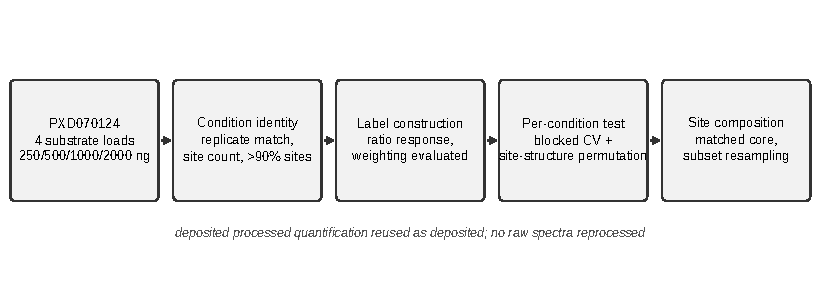
\includegraphics[width=\textwidth]{figures/figure1_reuse_workflow.pdf}

\caption{Reuse workflow. Site-level quantification deposited for four substrate loads is used as deposited; the condition reported by the published figure is identified, labels are constructed and the weighting scheme evaluated, the structure--response relationship is tested separately in each condition, and site composition is examined with a matched core and random-subset resampling.}\label{fig:workflow}\end{figure}

\subsection{An independent implementation reproduces the published condition}

Applied to the 500 ng condition under the weighting scheme of the source pipeline, the nine-descriptor representation reached a mean absolute error of 0.184 against a mean-predictor baseline of 0.300, with Spearman rank correlation 0.681 and a permutation-control advantage of 0.100 (P = 0.005). The corresponding published values for the same sites are 0.186, 0.699 and 0.113. The agreement establishes that the feature definitions, spatial blocking and permutation control reproduce the published behaviour, so the results that follow are not attributable to implementation differences.

\subsection{Label weighting determines whether the relationship is detected}

Inverse-variance weights derived from the delta-method variance are extremely skewed. Within a condition they span five orders of magnitude, from 0.0002 to 28.4 at the lowest load, and the Kish effective sample size falls to between 0.23 and 0.32 of the nominal site count: the thirty-three nominal sites of the published condition correspond to an effective sample of 9.7 (Table 2, Figure 2A and 2B).

The consequence is substantive. Under inverse-variance weighting the permutation-controlled signal was recovered in three of four conditions, failing at the lowest load (Spearman 0.141, $P$ = 0.109). Without weighting it was recovered in all four, and rank correlations were higher in three of the four conditions (Table 3, Figure 2C and 2D). Clipping the weights to a moderate range reproduced the weighted result rather than the unweighted one, which indicates that the difficulty is the direction of the weighting rather than a few extreme values.

The mechanism is specific to ratio-based response measures. The delta-method variance carries the control mean in its denominator, so sites with low control abundance receive large variances and correspondingly small weights. Low occupancy is a property of the site rather than noise about the structure-response relationship, so inverse-variance weighting systematically downweights low-occupancy sites. We therefore report unweighted analyses as primary.

\begin{figure}[htbp]\centering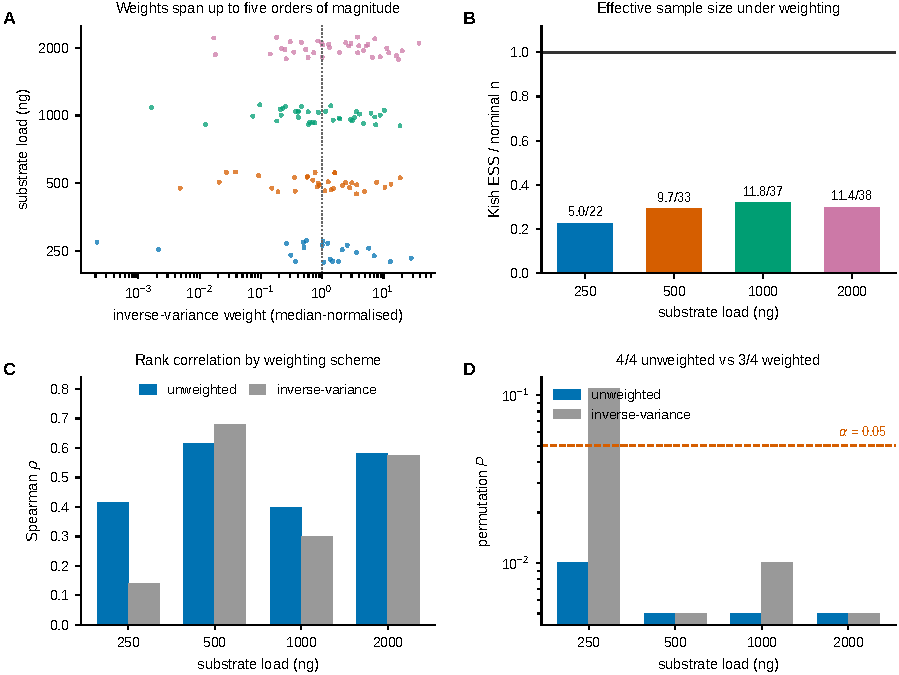
\includegraphics[width=\textwidth]{figures/figure2_label_weighting.pdf}

\caption{Label weighting governs whether the relationship is detected. (A) Inverse-variance weights, median-normalised, for each substrate load; the dotted line marks unit weight. (B) Kish effective sample size as a fraction of the nominal site count, with the raw values above each bar. (C) Spearman rank correlation under each weighting scheme. (D) Empirical permutation $P$ values on a logarithmic scale; the dashed line marks $\alpha = 0.05$.}\label{fig:weighting}\end{figure}

\subsection{The relationship replicates across all four substrate loads}

Unweighted, local structural descriptors carried permutation-controlled predictive information in every condition: empirical P values were 0.010, 0.005, 0.005 and 0.005 at 250, 500, 1000 and 2000 ng, with Spearman correlations of 0.414, 0.616, 0.399 and 0.581 and improvements over the mean predictor of 0.090, 0.102, 0.064 and 0.091 (Table 3). Three of the four reach the resolution limit of two hundred permutations; the observed errors lie below their permutation nulls in every condition (Figure 3A, 3B).

Extending the descriptor table to every lysine in the union across conditions contributed to this result. The table distributed with the original analysis covers only the thirty-three sites of the published condition; eleven lysines appearing at other loads were absent from it, not because of any structural or quality criterion but because the table was built for one condition. Including them raised the 1000 ng condition from P = 0.020 to P = 0.005 and the 250 ng condition from P = 0.030 to P = 0.010.

\subsection{Response dispersion does not explain the differences between conditions}

A natural explanation for a relationship appearing more strongly in some conditions than others is that response variation collapses in the weaker ones, leaving less to predict. The data do not support it. Response standard deviations were 0.357, 0.310, 0.304 and 0.298 across the four loads and interquartile ranges 0.574, 0.509, 0.533 and 0.492, a spread of at most twenty percent between the widest and narrowest condition. Mean response declined with increasing substrate load, from 0.602 at 500 ng to 0.455 at 2000 ng, which is the expected direction when enzyme concentration is held constant and substrate rises, and serves as a sanity check that the conditions behave as the design implies. The conditions differed mainly in where responses accumulated at the upper boundary, with seven sites above 0.90 at 500 ng against five, zero and one elsewhere, but total dispersion was comparable throughout.

\subsection{Site composition, not power, limits the relationship}

Twenty lysines passed the confidence threshold in all four conditions. Restricting every condition to this matched set removes site composition as a difference between conditions, and under that restriction no condition retained a permutation-controlled signal: P values were 0.080, 0.194, 0.264 and 0.129, and in the published condition the rank correlation became negative at -0.224 (Table 4).

Because reducing the sample also reduces power, we drew two hundred random twenty-site subsets of the published condition. Their mean Spearman correlation was 0.400, the median 0.461, and seventy-four percent exceeded 0.3; mean improvement over baseline was 0.062. Twenty sites therefore suffice to recover the relationship when drawn at random. The matched set reached -0.224 and a baseline improvement of 0.003, placing it at the third percentile (Figure 3C, 3D). Power is thus excluded as the explanation. We note that the random subsets are drawn from the same thirty-three sites and overlap the matched set substantially, so the reference distribution is not independent of it, and a third-percentile outcome arises by chance in roughly one draw in thirty; the comparison bounds the power explanation without establishing that the matched sites form a distinct class.

\begin{figure}[htbp]\centering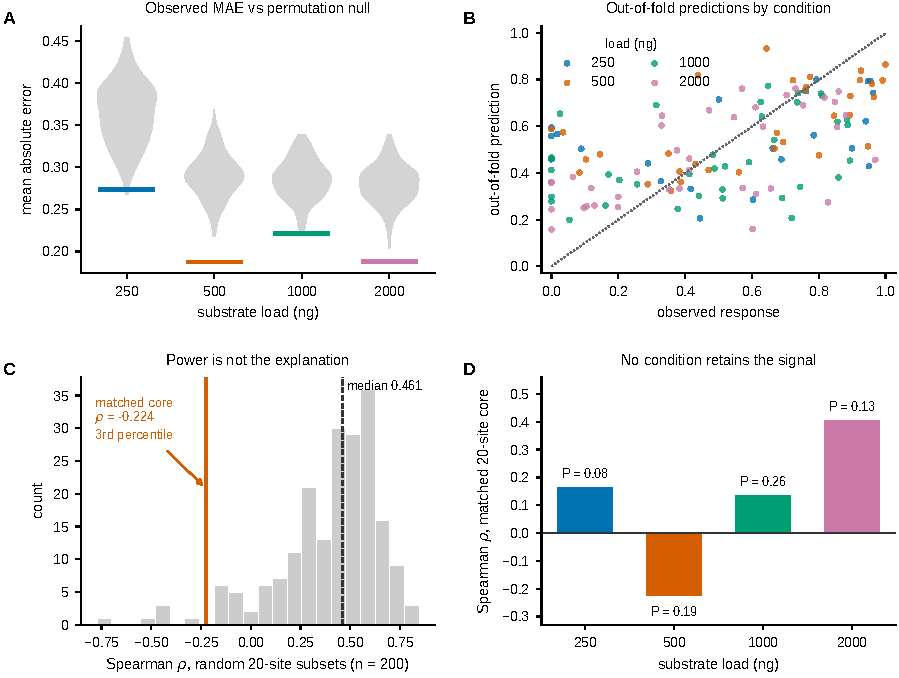
\includegraphics[width=\textwidth]{figures/figure3_replication_composition.pdf}

\caption{Condition replication and site composition. (A) Permutation null distributions of mean absolute error for each load (grey) with the observed value marked. (B) Out-of-fold predictions against observed response, by load; the dotted line is the identity. (C) Spearman correlations of 200 random twenty-site subsets of the 500 ng condition, with the median and the matched twenty-site core marked. (D) Spearman correlation on the matched core in each condition, with empirical $P$ values.}\label{fig:composition}\end{figure}

\subsection{Measurement confidence does not confound the relationship}

Structural descriptors did not predict in how many conditions a site was confidently quantified after correction for testing nine descriptors (Bonferroni threshold 0.0056); the strongest association was neighbourhood hydrophobic fraction (Spearman 0.442, P = 0.0101), which does not survive correction, and no descriptor was associated with mean confidence (all P > 0.11). Within the published condition, confidence score and response were unrelated (Spearman -0.087, P = 0.63). The matched and unmatched site groups had indistinguishable response distributions, with means of 0.602 and 0.603 (Mann-Whitney P = 0.84). Comparing the groups descriptor by descriptor gave no difference surviving correction, the smallest P value again belonging to neighbourhood hydrophobic fraction (0.404 against 0.251, P = 0.0164). We report the convergence of hydrophobic neighbourhood across two uncorrected tests as a lead, noting that it is the descriptor family the source study associated with reduced activity, and not as a finding.

\subsection{Discussion}

The object of this study is not an enzyme but a class of data. Site-resolved measurements of how a modification responds to a perturbation are beginning to be reused as quantitative labels, and the steps between an archive and a conclusion are numerous enough that the same deposition can support different answers. Working through those steps on one dataset, we found two that mattered enough to change the result, and both were encountered rather than anticipated.

The first and more general is label weighting. Defining a response as one minus the ratio of treated to control abundance makes a delta-method variance immediately available, and using it as an inverse-variance weight is the textbook response to heteroscedastic measurements. Here it was counterproductive. The weights spanned up to five orders of magnitude, the effective sample size fell to roughly a third of the nominal site count, and the structure-response relationship was recovered in three of four conditions weighted against four of four unweighted, with lower rank correlations in three of the four. That clipping the weights reproduced the weighted rather than the unweighted outcome locates the problem in the direction of the weighting, not in outliers. The mechanism is worth stating plainly because it is not specific to this dataset: the delta-method variance of a ratio carries the denominator mean in its own denominator, so sites with low control occupancy receive large variances and small weights. Low occupancy is a property of the site, not noise about the structure-response relationship, and downweighting those sites therefore discards signal rather than noise. We suggest that reuse of ratio-based site-level response labels treat inverse-variance weighting as a modelling choice that requires justification, and that unweighted and weighted analyses be reported alongside each other.

The second is condition identity, which is less deep but more easily fixed. The archive deposits four substrate loads; the published site-level figure reports one of them without saying which, and we identified it only by matching replicate values, site counts and the number of highly responsive sites. A secondary user who takes labels from that figure inherits both a condition and the set of lysines that happened to pass the confidence threshold at that condition, and the set differs appreciably between loads: twenty-two, thirty- three, thirty-seven and thirty-eight sites, with only twenty passing in all four. Stating the condition in the figure legend would cost nothing and would remove the ambiguity entirely. More broadly, when a deposition contains several conditions, a reuser should test across them rather than treat the published one as representative; in this case that test was available at no experimental cost and changed the conclusion.

With labels constructed accordingly, the biological question admits a clearer answer than the source report could give. Local structural descriptors carried permutation-controlled predictive information at all four substrate loads. This is informative about the source study's own internal tension: its Results text reported specific structural preferences, higher activity near cysteines and reduced activity near bulky hydrophobic or aromatic residues, while its figure legend stated that activity showed no clear preference based on primary or secondary structure. Our result supports the former reading. The preferences are real and detectable, they survive spatial blocking and a site-structure permutation control, and they reproduce across conditions, which a single-condition analysis cannot demonstrate. We emphasise that this is quantification and confirmation of hypotheses the source authors stated, not their discovery.

The relationship is nonetheless not uniform across sites, and we regard establishing that as part of the contribution rather than a shortfall. The twenty lysines quantified confidently at every load showed no permutation-controlled signal in any condition, and in the published condition the rank correlation was slightly negative. Random-subset resampling separates this from a power effect: three quarters of random twenty-site subsets of the published condition retained a rank correlation above 0.3, with a median of 0.461, so twenty sites suffice when drawn at random, and the matched set fell at the third percentile. What distinguishes those sites we cannot say. Measurement confidence does not predict response, the matched and unmatched groups have indistinguishable response distributions, and no descriptor separates them after correction for multiple testing. The one descriptor pointing consistently in the same direction across two uncorrected tests was neighbourhood hydrophobic fraction, which is the family the source study associated with reduced activity; with thirty-three sites and nine descriptors we report it as a lead and nothing more. We also note that the random subsets are drawn from the same thirty-three sites and overlap the matched set substantially, so the reference distribution is not independent of it, and a third-percentile outcome arises by chance in roughly one draw in thirty. The power explanation is excluded; the alternative, that the matched sites form a structurally distinct class, is not established.

A second and independent instability appeared when the frozen model was compared with the bulk responses the source study reported for casein, haemoglobin and collagen. The experimental ordering itself is consistent, casein exceeding haemoglobin and haemoglobin exceeding collagen at all three modification levels deposited with the source report, so the comparison does not fail on the measurement side. Under the prespecified specification it could not be made at all, because no collagen lysine satisfied both the structure-confidence and applicability-domain criteria; across the ninety-six of one hundred and ninety-two pipeline configurations in which all three scaffolds were represented, only seven recovered the reported ordering, against a chance expectation of one in six. These configurations are nested variants of a single pipeline and strongly correlated, so that fraction is descriptive rather than a test, and selecting the agreeing minority after the fact would be specification search. The mechanistic reading is straightforward: monomeric predicted structures do not represent a casein micelle, the subunit interfaces of a haemoglobin tetramer or a collagen triple helix, and a bulk immunoassay endpoint does not identify which lysines carried the modification. We also note a hard limit on what this comparison could ever have shown, since with three scaffolds an exact-ordering test cannot yield a p-value below one in six.

Two boundaries define how these results should be used. All labelled sites come from a single protein and a single assay, so spatial blocking reduces leakage between neighbouring lysines but cannot create protein-level independence, and nothing here licenses extrapolation to other scaffolds; the cross-scaffold comparison above is direct evidence of that boundary rather than an argument against it. And the four substrate loads are conditions within one experiment, so agreement across them establishes robustness to substrate load rather than independent biological replication, which is the sense in which we use the term throughout.

Sample size shapes the reporting rather than the conclusions. With twenty-two to thirty-eight sites per condition we report permutation-controlled error differences and rank correlations rather than coefficients of determination, which are unreliable at this scale, and we have refrained from interpreting the ordering of conditions or from assigning causal roles to individual descriptors. No public site-resolved response dataset exists for a second protein, so the external comparison available to us was necessarily at protein level; that gap is a property of the field at present rather than of this analysis, and it defines what would most advance the question.

These limitations point to a specific next experiment rather than to a larger model. What is needed is a prespecified panel of structurally diverse proteins, measured at modified-lysine resolution under a shared active-versus-inactive protocol and at more than one substrate load, with the condition reported. Such a panel would also make it worthwhile to move beyond the single crystallographic model used here toward conformational ensembles and native assemblies, which the present descriptors do not represent. Measuring more than one load is the inexpensive part and, on the evidence here, the part that determines whether a structure-response relationship inferred from such data can be trusted.

\begin{suppinfo}

The Supporting Information is available free of charge at the publisher's website.

\par Protein-level comparison with bulk responses, including Figure~S1; response dispersion by substrate load (Table~S1); descriptor extraction and validation (PDF).

\end{suppinfo}

\section*{Author Information}

\textbf{Corresponding Author.} Murat G\"ok --- Department of Computer Engineering, Faculty of Engineering, Yalova University, 77200 Yalova, T\"urkiye; ORCID 0000-0003-2261-9288; Email: murat.gok@yalova.edu.tr

\textbf{Author Contributions.} M.G. is the sole author. M.G. conceived the study, designed and implemented the analyses, prepared the figures and tables, and wrote the manuscript.

\textbf{Notes.} The author declares no competing financial interest.

\section*{Data and Code Availability}

All data analysed here are publicly deposited. Site-level quantification was obtained from ProteomeXchange PXD070124; the four source files are identified by SHA-256 in Table~1. Structural coordinates are from PDB 4F5S. Code, derived label tables, configurations and result files are available at \url{https://github.com/murat-gok/cml-repairnet}.

\begin{acknowledgement}

The author thanks the investigators who generated and openly shared the carboxymethyllysine proteomics datasets reused here.

\end{acknowledgement}

\bibliography{references_jpr}

\end{document}
